\subsection{Generazione Immagini Corrotte}
\textbf{Obiettivo:}
Degradare le immagini applicando, mediante le funzioni riportate nella cella precedente,  l'operatore di blur con parametri
\begin{itemize}
    \item{$\sigma=0.5$ dimensione $5\times 5$}
    \item{$\sigma=1$ dimensione $7\times 7$}
    \item{$\sigma=1.3$ dimensione $9\times 9$}
\end{itemize}
ed aggiunge rumore gaussiano con deviazione standard (0, 0.05)

\begin{figure}[H]
    \centering
    \begin{minipage}[h]{0.5\textwidth}
        \centering
    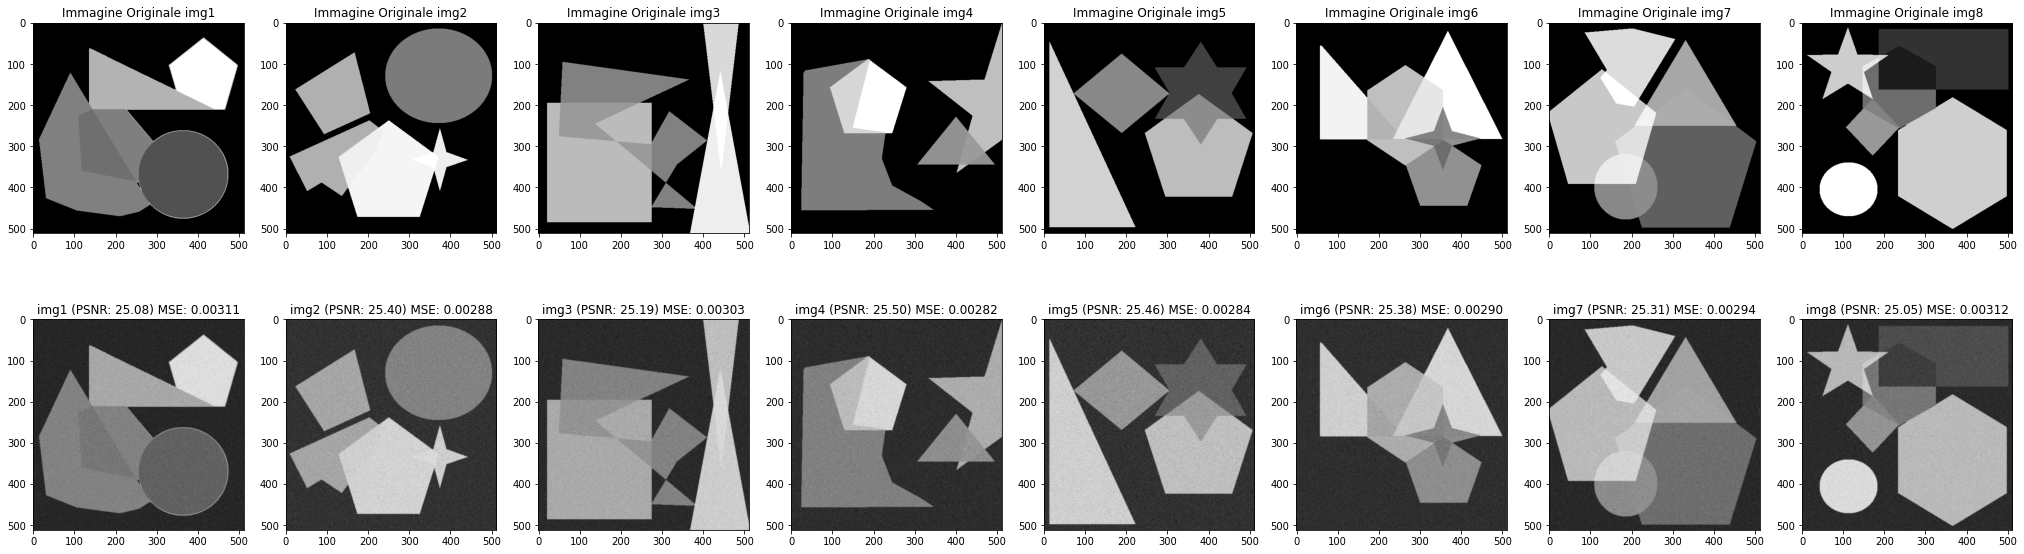
\includegraphics[width=\linewidth]{imgRel/datasetcorrotto/datasetcorrotto5x5.png}\label{fig:imgcorrotte1}
    \end{minipage}%
    \begin{minipage}[h]{0.5\textwidth}
        \centering
        \begin{tabular}{|lr|}
        \hline
        \multicolumn{1}{|c}{\textbf{Valore}} & \multicolumn{1}{c|}{\textbf{Risultato}} \\ \hline
        Media PSNR                           & 25.3137                                 \\
        Media MSE                            & 0.002943                                \\
        Dev. Std. PSNR                       & 0.156402                                \\
        Dev. Std. MSE                        & 0.000106                                \\ \hline
        \end{tabular}\label{tab:tabcorrotte1}
    \end{minipage}
    \captionlistentry[table]{Table corrotte}
    \captionsetup{labelformat=andtable}
    \caption{Immagini corrotte con $\sigma = 0.5$ dimensione $5 \times 5$}
\end{figure}

\begin{figure}[H]
    \centering
    \begin{minipage}[h]{0.5\textwidth}
        \centering
    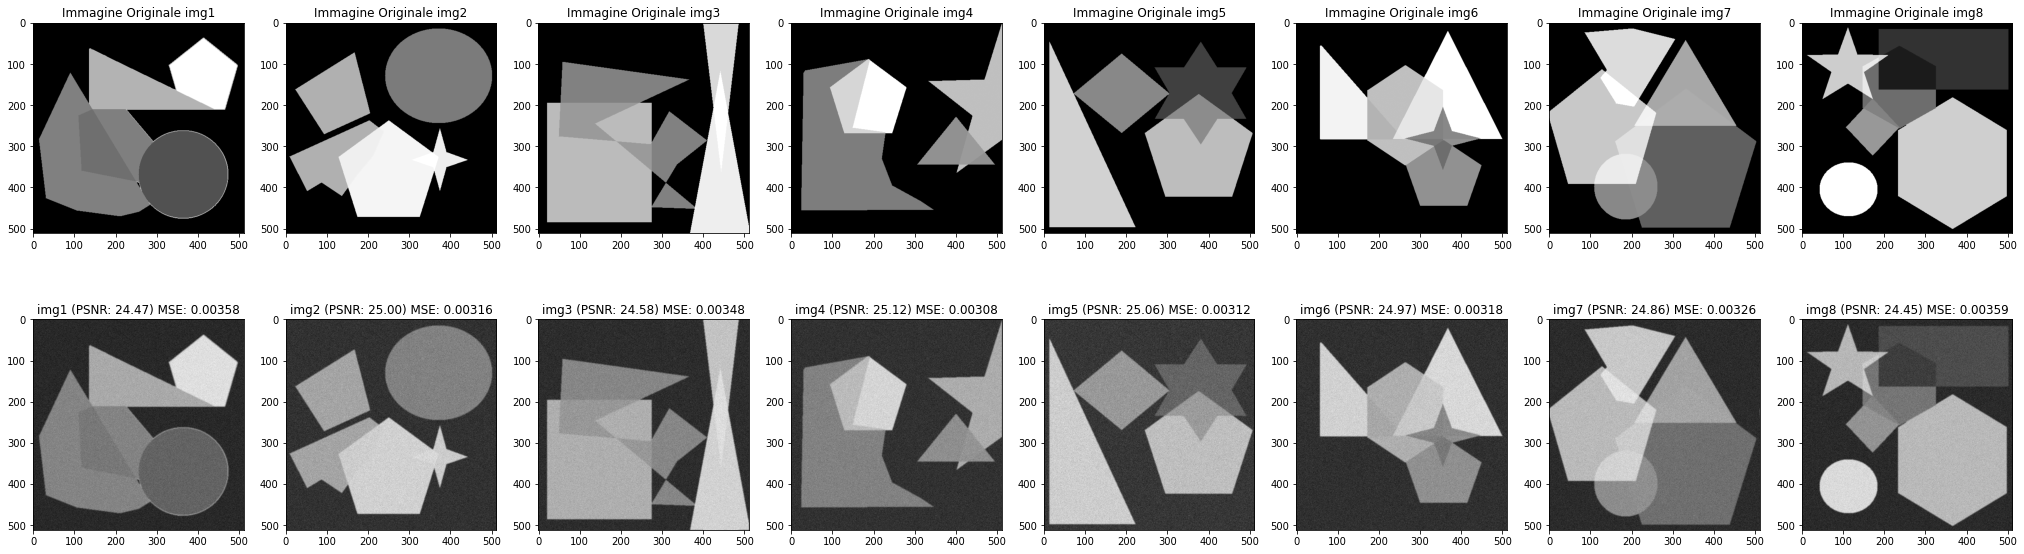
\includegraphics[width=\linewidth]{imgRel/datasetcorrotto/datasetcorrotto7x7.png}\label{fig:imgcorrotte2}
    \end{minipage}%
    \begin{minipage}[h]{0.5\textwidth}
        \centering
        \begin{tabular}{|lr|}
            \hline
            \multicolumn{1}{|c}{\textbf{Valore}} & \multicolumn{1}{c|}{\textbf{Risultato}} \\ \hline
                Media PSNR & 24.7938 \\ 
                Media MSE & 0.003321 \\ 
                Dev. Std. MSE & 0.000194 \\ 
                Dev. Std. PSNR & 0.252202 \\ \hline
            \end{tabular}\label{tab:tabcorrotte2}
    \end{minipage}
    \captionlistentry[table]{Table corrotte}
    \captionsetup{labelformat=andtable}
    \caption{Immagini corrotte con $\sigma = 1$ dimensione $7 \times 7$}
\end{figure}

\begin{figure}[H]
    \centering
    \begin{minipage}[h]{0.5\textwidth}
        \centering
    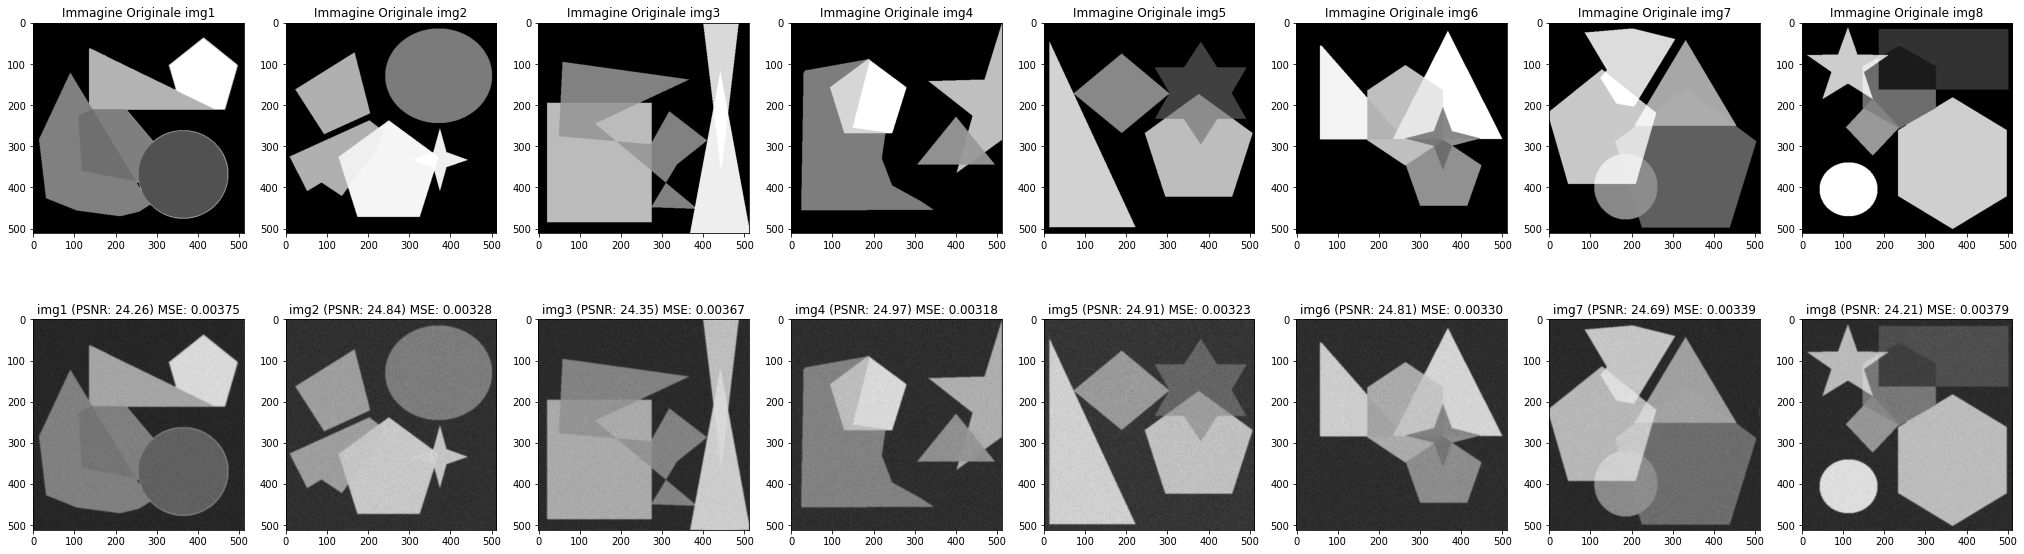
\includegraphics[width=\linewidth]{imgRel/datasetcorrotto/datasetcorrotto9x9.png}\label{fig:imgcorrotte3}
    \end{minipage}%
    \begin{minipage}[h]{0.5\textwidth}
        \centering
        \begin{tabular}{|lr|}
            \hline
            \multicolumn{1}{|c}{\textbf{Valore}} & \multicolumn{1}{c|}{\textbf{Risultato}} \\ \hline
                Media PSNR & 24.6292 \\ 
                Media MSE & 0.003452 \\ 
                Dev. Std. MSE & 0.000235 \\ 
                Dev. Std. PSNR & 0.293261 \\ \hline
            \end{tabular}\label{tab:tabcorrotte3}
    \end{minipage}
    \captionlistentry[table]{Table corrotte}
    \captionsetup{labelformat=andtable}
    \caption{Immagini corrotte con $\sigma = 1.3$ dimensione $9 \times 9$}
\end{figure}
